\documentclass[10pt,a4paper,twocolumn]{article}

% Packages
\usepackage[utf8]{inputenc}
\usepackage[T1]{fontenc}
\usepackage{amsmath}
\usepackage{amssymb}
\usepackage{amsthm}
\usepackage{graphicx}
\usepackage{hyperref}
\usepackage{geometry}
\usepackage{pgfplots}
\usepackage{xcolor}
\usepackage{sectsty}
\usepackage{quiver}
\usepackage{mathtools}
% Latin Modern fonts (includes sans-serif)
\usepackage{lmodern}

\pgfplotsset{compat=1.18}

% Page color
\definecolor{pagecolor}{HTML}{FAF9F6}
\pagecolor{pagecolor}

% Use sans-serif font throughout
\renewcommand{\familydefault}{\sfdefault}

% Make section headings sans-serif and bold
\allsectionsfont{\sffamily\bfseries}

\geometry{
    a4paper,
    left=20mm,
    right=20mm,
    top=25mm,
    bottom=25mm,
    columnsep=7mm
}

% Paragraph spacing
\setlength{\parskip}{0.5em}
\setlength{\parindent}{0pt}

% Title information
\title{
    
\includegraphics[width=3cm]{assets/botanix.png} \\
    \Huge \textbf{DynaFed Whitepaper}
}

\author{
    Fabio Lama\\
    \small BotanixLabs\\
    \small fabio@botanixlabs.xyz
    \and
    Darius Parvin\\
    \small BotanixLabs\\
    \small darius@botanixlabs.xyz
}
\date{
    \vspace{1em}
    \today \\
    \small
    \text{Revision 1 / Proof-of-Concept} \\[1em]
    \textit{Edited \& refined by:}\\Claude.ai (Anthropic) \\[2em]
    \footnotesize
    \textcopyright{} 2025 BotanixLabs \\
    \href{https://creativecommons.org/licenses/by/4.0/}{CC BY 4.0}
}

\begin{document}

\maketitle

\vspace*{1em}
\begin{abstract}
    DynaFed is a dynamic federation management protocol designed to enable secure and efficient Bitcoin custody for the Botanix layer 2 network. The protocol addresses the fundamental tension between security and operational efficiency in FROST threshold signature schemes by introducing a two-tier architecture: Tier 1 pools serve as large, conservative cold storage federations holding the majority of bridged funds, while Tier 2 pools operate as smaller, more flexible hot wallets optimized for low-latency withdrawal fulfillment. FROST's multi-round coordination protocol and static membership requirements create scalability bottlenecks that would be prohibitive for a single large federation, necessitating this architectural separation. DynaFed dynamically directs Bitcoin deposits and withdrawals based on real-time collateralization levels and network demand, using adaptive capacity estimation to adjust hot wallet reserves to changing withdrawal patterns. The system leverages Bitcoin's transaction output model as a core safeguard for operation atomicity and employs a lightweight fork-awareness algorithm that enables deterministic finality detection without external oracles. By maintaining collateralized hot wallets backed by cold storage reserves, DynaFed achieves a balance between the security guarantees of large federations and the operational responsiveness required for a production Bitcoin layer 2 network.
\end{abstract}

\clearpage
\tableofcontents
\clearpage

% Include section files
\section{Introduction}
\label{sec:introduction}

Botanix is an EVM-compatible layer 2 blockchain built on the Bitcoin network. Unlike most layer 2 systems that introduce new cryptocurrencies, Botanix employs a 1-to-1 peg with Bitcoin: users mint tokens by constructing a \textbf{pegin} through a verified Bitcoin transaction, and withdraw funds by constructing a \textbf{pegout} that burns tokens on Botanix and triggers a corresponding Bitcoin transaction.

Bitcoin's limited state introspection capabilities make it very hard to implement smart contracts that hold Bitcoin on behalf of external networks or validate their state transitions natively. This fundamental constraint drives the complexity addressed in this work: designing a secure, permissionless multisig system using FROST threshold signatures that can custody Bitcoin funds while maintaining the security and operational requirements of a production layer 2 network. The coordination complexity inherent to FROST, particularly its multi-round signing protocol and static membership requirements, fundamentally shapes our architectural decisions.

Botanix operates through three coordinated state layers, each producing cryptographic commitments that validators use to verify system-wide consistency:

\begin{itemize}
    \item \textbf{CometBFT}: Provides Byzantine Fault Tolerant consensus for block producer selection and transaction ordering
    \item \textbf{Application Layer}: Executes transactions and maintains deterministic EVM state, producing an EVM state commitment
    \item \textbf{Foundation Layer}: Coordinates multisig federation membership, pegout lifecycle management, and Bitcoin fork awareness, producing a Foundation state commitment
\end{itemize}

The Foundation Layer, which is the primary focus of this paper, addresses two key challenges: managing federation rotations despite FROST's static membership requirements, and tracking pegouts across Bitcoin's probabilistic finality model where chain reorganizations can "undo" previously confirmed transactions. These constraints motivate the two-tier federation architecture that balances security and operational flexibility.

\subsection{Document Structure}

This paper is organized into the following sections:

\begin{enumerate}
    \item \textbf{FROST Challenges \& Two-Tier Architecture}: Section \ref{sec:frost-challenge} describes the challenges inherent to the FROST protocol and motivates our two-tier federation system. Section \ref{sec:two-tier-federations} presents the architecture and analyzes the security-efficiency tradeoffs.
    \item \textbf{Pool Management}: Section \ref{sec:pool-management} presents the theory behind pegin and pegout allocation, defining how we balance the two-tier federation system securely and reliably.
          \begin{itemize}
              \item \textbf{Dynamic capacity targeting} (section \ref{sec:dynamic-capacity-target}): Maintains sufficient liquid funds in Tier 2 federations by adapting to pegout demand patterns
              \item \textbf{Real-time collateralization} (section \ref{sec:collateralization-level}): Ensures fund safety by tracking collateral backing for Tier 2 federations, mitigating risks from their smaller size
          \end{itemize}
    \item \textbf{Risk Assessment \& Lifecycle}: Section \ref{sec:risk-assessment} describes how DynaFed determines when new Tier 1 or Tier 2 federations must be established and how funds should be safely rotated to newly established federations.
          \begin{itemize}
              \item We define a reproducible risk metric that governs rotation urgency, favoring a conservative approach unless degradation is detected
          \end{itemize}
    \item \textbf{Pegout Proposals \& Bitcoin Finality}: Section \ref{sec:pegout-proposals} addresses the challenges of tracking pegout proposals once federation members construct Bitcoin L1 transactions.
          \begin{itemize}
              \item We examine how "executed" pegouts should be tracked across Bitcoin's probabilistic finality model and identify which assumptions cannot be made
              \item We leverage the UTXO-reuse property to prevent double-execution of pegouts in cases of orphaned Bitcoin blocks (where transactions return to mempool), proposal upgrades/fee bumps (section\ref{sec:pegout-proposal-upgrade}), or cancellations (section \ref{sec:pegout-proposal-cancellation})
              \item We present a lightweight Bitcoin fork awareness mechanism (section \ref{sec:bitcoin-fork-awareness}) that tracks pegout proposals across competing forks and orphaned blocks, enabling deterministic finality detection despite Bitcoin's probabilistic consensus
          \end{itemize}
    \item \textbf{Foundation Layer Integration}: Section \ref{sec:foundation-layer} describes the main component that coordinates all subsystems. The Foundation Layer interprets Botanix-specific consensus messages and orchestrates:
          \begin{itemize}
              \item Pegin and pegout routing decisions
              \item Dynamic capacity target and real-time collateralization calculations
              \item Risk metric computation and federation lifecycle management (construction, rotation, sunset)
              \item Bitcoin block and pegout proposal tracking with fork awareness
          \end{itemize}
\end{enumerate}

\begin{figure*}[t]
    \centering
    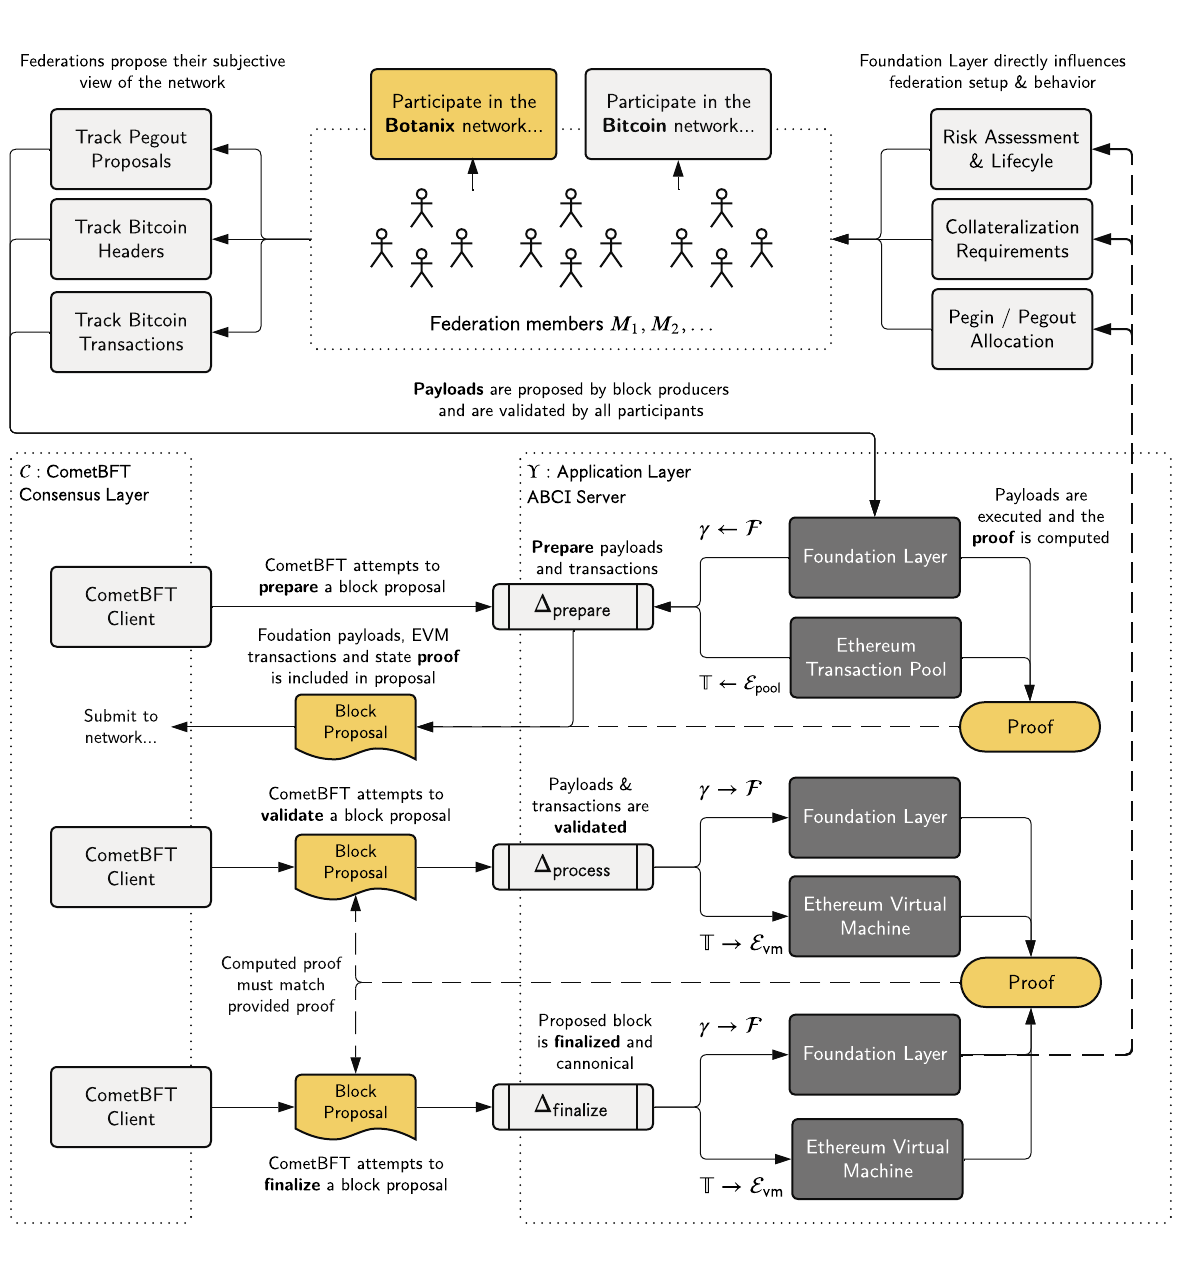
\includegraphics[width=\textwidth]{assets/dynafed_overview.png}
    \caption{DynaFed System Architecture}
    \label{fig:dynafed-overview}
\end{figure*}

\clearpage
\section{Architecture}
\label{sec:overview}

The consensus engine is the core component of any permissionless blockchain system. Botanix uses CometBFT, one of the most adopted and robust Proof-of-Stake (PoS) engines, which acts as middleware between arbitrary application logic and the consensus layer. While CometBFT follows its own specification, it provides sufficient flexibility for us to control transaction structure, state transition interpretation, and validator selection decisions. CometBFT treats application logic as a black box; from its perspective, both transactions and their resulting state transitions are opaque.

CometBFT operates as a standalone client $\mathcal{C}$ that communicates directly with other CometBFT clients, handling all consensus networking internally. However, because it is application-agnostic, CometBFT delegates transaction processing and state management to the application layer through the ABCI interface $\Delta$. The application logic $\Upsilon$ implements a handful of ABCI methods that the client uses to prepare block proposals, validate proposals, and finalize blocks.

\begin{center}
    % https://q.uiver.app/#q=WzAsNixbMiwyLCJcXG1hdGhjYWx7Q31fMSJdLFszLDMsIlxcbWF0aGNhbHtDfV8zIl0sWzAsMiwiXFxVcHNpbG9uXzEiXSxbMywxLCJcXG1hdGhjYWx7Q31fMiJdLFs0LDAsIlxcVXBzaWxvbl8yIl0sWzQsNCwiXFxVcHNpbG9uXzMiXSxbMCwzLCJcXHRleHRpdHtDb21ldEJGVH1cXFxcIFxcdGV4dGl0e1AyUH0iLDAseyJsYWJlbF9wb3NpdGlvbiI6NDAsImxldmVsIjoyLCJzdHlsZSI6eyJ0YWlsIjp7Im5hbWUiOiJhcnJvd2hlYWQifX19XSxbMCwxLCIiLDEseyJsZXZlbCI6Miwic3R5bGUiOnsidGFpbCI6eyJuYW1lIjoiYXJyb3doZWFkIn19fV0sWzEsMywiIiwxLHsibGV2ZWwiOjIsInN0eWxlIjp7InRhaWwiOnsibmFtZSI6ImFycm93aGVhZCJ9fX1dLFszLDQsIlxcRGVsdGFfe1xcY2RvdHN9IiwxLHsic3R5bGUiOnsidGFpbCI6eyJuYW1lIjoiYXJyb3doZWFkIn19fV0sWzEsNSwiXFxEZWx0YV97XFxjZG90c30iLDEseyJzdHlsZSI6eyJ0YWlsIjp7Im5hbWUiOiJhcnJvd2hlYWQifX19XSxbMCwyLCJcXERlbHRhX3tcXGNkb3RzfSIsMSx7InN0eWxlIjp7InRhaWwiOnsibmFtZSI6ImFycm93aGVhZCJ9fX1dLFs0LDUsIiIsMSx7InN0eWxlIjp7InRhaWwiOnsibmFtZSI6ImFycm93aGVhZCJ9fX1dLFs0LDIsIlxcdGV4dGl0e0V0aGVyZXVtfVxcXFwgXFx0ZXh0aXR7UDJQfSIsMix7ImxhYmVsX3Bvc2l0aW9uIjo4MCwiY3VydmUiOjUsInN0eWxlIjp7InRhaWwiOnsibmFtZSI6ImFycm93aGVhZCJ9fX1dLFs1LDIsIiIsMSx7ImN1cnZlIjotNSwic3R5bGUiOnsidGFpbCI6eyJuYW1lIjoiYXJyb3doZWFkIn19fV1d
    \begin{tikzcd}
        &&&& {\Upsilon_2} \\
        &&& {\mathcal{C}_2} \\
        {\Upsilon_1} && {\mathcal{C}_1} \\
        &&& {\mathcal{C}_3} \\
        &&&& {\Upsilon_3}
        \arrow["\begin{array}{c} \textit{Ethereum}\\ \textit{P2P} \end{array}"'{pos=0.8}, curve={height=30pt}, tail reversed, from=1-5, to=3-1]
        \arrow[tail reversed, from=1-5, to=5-5]
        \arrow["{\Delta_{\cdots}}"{description}, tail reversed, from=2-4, to=1-5]
        \arrow["\begin{array}{c} \textit{CometBFT}\\ \textit{P2P} \end{array}"{pos=0.4}, Rightarrow, 2tail reversed, from=3-3, to=2-4]
        \arrow["{\Delta_{\cdots}}"{description}, tail reversed, from=3-3, to=3-1]
        \arrow[Rightarrow, 2tail reversed, from=3-3, to=4-4]
        \arrow[Rightarrow, 2tail reversed, from=4-4, to=2-4]
        \arrow["{\Delta_{\cdots}}"{description}, tail reversed, from=4-4, to=5-5]
        \arrow[curve={height=-30pt}, tail reversed, from=5-5, to=3-1]
    \end{tikzcd}

    \vspace{0.5em}
    \small{Three validators communicating, where each pair $(\mathcal{C}_n, \Upsilon_n)$ represents a complete validator node. $\mathcal{C}_n$ is the CometBFT consensus client and $\Upsilon_n$ is the application layer.}
\end{center}

Since Botanix is an EVM-compatible chain, we reuse Ethereum's execution layer while replacing Ethereum's native consensus with CometBFT. Currently, all network participants (validators and non-validators alike) must run the CometBFT client, which handles transaction gossiping and block finalization. Ethereum's P2P block propagation is disabled in favor of CometBFT's networking layer. Future protocol versions may revisit this architecture to allow non-validators to sync via alternative mechanisms.

The most significant ABCI interfaces that $\Upsilon$ must implement are $\Delta_{\text{prepare}}$, $\Delta_{\text{process}}$, and $\Delta_{\text{finalize}}$. The consensus client $\mathcal{C}$ invokes each interface according to its internal specification and the current consensus state.

\[
    \mathcal{C} \mathrel{\substack{\longrightarrow \\ \longleftarrow}}
    \left\{
    \begin{aligned}
         & \Delta_{\text{prepare}}  &  & \text{construct block proposal} \\
         & \Delta_{\text{process}}  &  & \text{validate proposed block}  \\
         & \Delta_{\text{finalize}} &  & \text{commit finalized block}   \\
         & \Delta_{\cdots}          &  & \cdots
    \end{aligned}
    \right\}
    \mathrel{\substack{\longrightarrow \\ \longleftarrow}} \Upsilon
\]

An important aspect of CometBFT is that it establishes consensus on transactions, not blocks. This means that state changes must be perfectly reproducible from the agreed-upon list and order of transactions. To support Botanix-specific coordination logic, we reserve the first transaction slot in every block for \textbf{Non-Deterministic Data} (NDD), denoted $\gamma$. This special transaction is constructed by the block producer and executed by the \textbf{Foundation Layer} $\mathcal{F}$. It contains off-chain coordination messages that cannot be derived deterministically from prior state alone, but is still validated according to $\mathcal{F}$'s consensus rules. The last element in $\gamma$ is always the \textbf{Foundation state proof} $\mathcal{F}^{\Phi}$, as defined in section~\ref{sec:foundation-state-proof-structure}:

\[
    \gamma_{|\gamma|} = \mathcal{F}^{\Phi}
\]

The Foundation Layer is described in more detail in section \ref{sec:foundation-layer}.

\subsection{Block Proposal Construction}

When $\mathcal{C}$ decides to construct a block proposal by calling $\Delta_{\text{prepare}}$ on $\Upsilon$, the endpoint combines two distinct sources: the Foundation Layer produces $\gamma$, while the standard Ethereum transaction pool $\mathcal{E}_{\text{pool}}$ provides user transactions. The resulting proposal always places $\gamma$ first:

\begin{center}
    \begin{equation*}
        \begin{aligned}
             & \lambda[\gamma, \mathbb{T}] \leftarrow \Upsilon.\Delta_{\text{prepare}} :=
            \begin{cases}
                \gamma \leftarrow \mathcal{F}                   \\
                \texttt{rollback}(\mathcal{F})                  \\
                \mathbb{T} \leftarrow \mathcal{E}_{\text{pool}} \\
                \texttt{return } [\gamma, \mathbb{T}]
            \end{cases}                              \\
             & \quad \text{where } \mathbb{T} = [t_i]_{i=1}^n
        \end{aligned}
    \end{equation*}

    \vspace{0.5em}
    \small{Note: \texttt{rollback()} discards tentative state changes and returns to the previous block's state. This allows validation to occur without persisting changes until finalization.}
\end{center}

The function returns a CometBFT-constructed structure $\lambda$ that includes additional consensus-related information (validator selection, evidence of equivocation, etc.), with the NDD $\gamma$ at position zero followed by an ordered list of transactions $\mathbb{T}$, which may be empty. The EVM state proof $\mathcal{E}_{\text{vm}}^{\Phi}$ is placed in the structure's \textit{appHash} field, following standard CometBFT convention. The Foundation state proof $\mathcal{F}^{\Phi}$ is embedded in the Ethereum block's \textbf{extra data header}, making it part of $\mathcal{E}_{\text{vm}}^{\Phi}$. Consequently, both proofs are transitively committed in the \textit{appHash}.

Formally:
\[
    \{\mathcal{E}_{\text{vm}}^{\Phi}, \mathcal{F}^{\Phi}\} \subseteq \lambda.\textit{appHash}
\]

\subsection{Block Proposal Validation \& Finalization}

When $\mathcal{C}$ receives a block proposal $\lambda[\gamma, \mathbb{T}]$ from a peer, it submits the proposal to the $\Delta_{\text{process}}$ validation function of $\Upsilon$. The validation process first extracts and validates $\gamma$ (which must be present), passing it to the Foundation Layer for verification. The remaining transactions $\mathbb{T}$ are then passed to the Ethereum EVM $\mathcal{E}_{\text{vm}}$ for standard execution validation:

\begin{equation*}
    \begin{aligned}
         & \begin{rcases}
               \lambda[\gamma, \mathbb{T}] & \rightarrow \\
               f                           & \leftarrow
           \end{rcases}
        \Upsilon.\Delta_{\text{process}} :=
        \begin{cases}
            \gamma \rightarrow \mathcal{F}                 \\
            \mathbb{T} \rightarrow \mathcal{E}_{\text{vm}} \\
            \texttt{rollback}(\mathcal{E}_{\text{vm}})     \\
            \texttt{rollback}(\mathcal{F})                 \\
            \texttt{return } f
        \end{cases}                                     \\
         & \quad \text{where } \mathcal{C} \text{ validates } \lambda.\texttt{appHash}\stackrel{?}{=}f.\texttt{appHash}
    \end{aligned}
\end{equation*}

where $f$ is a validation result indicating whether the proposal is accepted or rejected by the consensus rules. A block is only considered \textbf{canonical} (i.e., finalized) after $\mathcal{C}$ calls $\Delta_{\text{finalize}}$, which replicates the behavior of $\Delta_{\text{process}}$ with the critical exception that state changes are now \textbf{committed} (persisted and canonical) rather than rolled back:

\begin{equation*}
    \begin{aligned}
        \begin{rcases}
            \lambda[\gamma, \mathbb{T}] & \rightarrow \\
            f                           & \leftarrow  \\
        \end{rcases}
        \Upsilon.\Delta_{\text{finalize}} :=
        \begin{cases}
            \gamma \rightarrow \mathcal{F}                 \\
            \texttt{commit}(\mathcal{F})                   \\
            \mathbb{T} \rightarrow \mathcal{E}_{\text{vm}} \\
            \texttt{commit}(\mathcal{E}_{\text{vm}})       \\
            \texttt{return } f
        \end{cases}
    \end{aligned}
\end{equation*}

\subsection{System Flow: Pegin Lifecycle}

When a user deposits Bitcoin into Botanix:

\begin{enumerate}
    \item User constructs a Bitcoin transaction sending funds to a multisig address controlled by either a Tier 1 or Tier 2 pool
    \item DynaFed routing logic (section \ref{sec:pegin-allocation-logic}) determines the destination based on:
          \begin{itemize}
              \item Dynamic capacity target $H(t)$ (section \ref{sec:dynamic-capacity-target})
              \item Current collateralization levels of Tier 2 pools (\ref{sec:collateralization-level})
              \item Risk-adjusted collateral availability (\ref{sec:risk-assessment})
          \end{itemize}
    \item Once the Bitcoin transaction achieves sufficient confirmations, the Foundation Layer registers it
    \item The EVM layer mints corresponding tokens to the user's Botanix address
\end{enumerate}

\subsection{System Flow: Pegout Lifecycle}

When a user withdraws Bitcoin from Botanix:

\begin{enumerate}
    \item User burns tokens on the EVM layer via a dedicated smart contract, triggering a pegout request
    \item The Foundation Layer records the pegout as \textbf{unassigned} with a list of qualified candidate pools
    \item DynaFed's pegout allocation logic (section \ref{sec:pool-management}) selects which Tier 2 pool(s) should fulfill the request based on:
          \begin{itemize}
              \item Collateralization deficits (priority to under-collateralized pools)
              \item Load distribution across healthy pools
              \item Risk assessment scores (section \ref{sec:risk-assessment})
              \item Fallback to Tier 1 pool if the amount exceeds funds
          \end{itemize}
    \item The selected pool's representative submits a \textbf{proposal} to the Foundation Layer (section \ref{sec:pegout-proposals}), coupling the pegout with specific UTXOs
    \item Pool members coordinate off-chain via FROST to sign the Bitcoin transaction
    \item Once the transaction appears in a Bitcoin block and achieves finality depth, the Foundation Layer classifies it as \textbf{finalized}
    \item The block tree pruning algorithm (section \ref{sec:block-tree}) automatically handles any Bitcoin forks
\end{enumerate}

\section{The FROST Challenge}
\label{sec:frost-challenge}

The FROST threshold signature protocol presents a fundamental scalability challenge for federation design. DKG setup requires multiple rounds of package exchanges between all participants, creating significant coordination overhead. While DynaFed can schedule DKG processes asynchronously where timing is less critical, the two-round signing protocol for pegout fulfillment remains a bottleneck, with larger federations facing increased message complexity, higher failure rates, and greater coordination burden.

This creates a tension between security and operational efficiency. Larger federations provide stronger security guarantees but struggle with FROST's coordination requirements. Smaller federations operate more efficiently but offer weaker security and are more vulnerable to attacks.

To address this tradeoff, we propose a two-tier federation system as described in section \ref{sec:two-tier-federations}. Tier 1 serves as a large ``cold wallet'' responsible for holding the majority of funds with maximum security. Tier 2 operates as a smaller ``hot wallet'' optimized for responsive pegout fulfillment. This separation allows each tier to play to its strengths: Tier 1 prioritizes security through size, while Tier 2 prioritizes operational efficiency through agility.

See appendix \ref{appendix:dkg-message-complexity} for a detailed breakdown of message complexity.

\section{Two-Tier Federations}
\label{sec:two-tier-federations}

We generally want funds to be as secure as possible, which suggests keeping them in the largest federation practical. However, larger federations have drawbacks: increased message complexity, reduced flexibility, and higher failure rates for operations like DKG processes and pegout signing requests as expanded on in section \ref{sec:frost-challenge}.

Fortunately, we can leverage a key observation: the majority of funds remain dormant with minimal movement, while only a small subset is actively used for pegouts. This allows us to structure a system that addresses both security and operational efficiency requirements:

\begin{itemize}
    \item \textbf{Tier 1} serves as the larger ``cold wallet'' where the majority of funds remain secured
    \item \textbf{Tier 2} serves as the smaller ``hot wallet'' responsible for honoring pegouts
\end{itemize}

DynaFed ensures that Tier 2 funds are substantially collateralized on Tier 1, \emph{ideally} at 100\%. This collateralization model provides several benefits:

\begin{itemize}
    \item \textbf{Reduced risk}: Tier 2 failures have limited impact due to collateral backing
    \item \textbf{Increased flexibility}: We can experiment with different federation sizes, collateralization requirements, and rotation schedules for Tier 2
    \item \textbf{Lower barriers}: We can accept newer or less-established CometBFT validators into Tier 2
\end{itemize}

\textbf{Note:} While we generally refer to Bitcoin multisigs as federations, we'll adopt the term \textbf{pools} going forward, which aligns better with how the broader crypto and DeFi ecosystem conceptualizes fund movements and custody.

\subsection{Tier 1 Architecture}

Tier 1 serves as the primary cold storage federation, holding the majority of bridged funds with maximum security guarantees. DynaFed maintains \textbf{exactly one active Tier 1 federation} under normal operation, though multiple Tier 1 pools may temporarily coexist during migration periods when an old pool  is being sunset in favor of a new pool.

The Tier 1 federation is intentionally large and conservative in its membership. DynaFed selects the most reliable, established, and senior members of the CometBFT validator set for this critical role. This selection bias reflects the security-first mandate of cold storage:

\begin{itemize}
    \item \textbf{High barriers to entry}: New validators face significant hurdles to joining Tier 1, requiring demonstrated reliability and stake history
    \item \textbf{Membership stability}: Established Tier 1 members are rarely removed unless they exhibit clear unreliability or misconduct
    \item \textbf{Reputation weighting}: Long-standing validators with proven track records receive priority over newer participants
\end{itemize}

This conservative approach prioritizes security and stability over operational flexibility, which is appropriate given that Tier 1 holds the bulk of user funds. Validators seeking to participate in the federation typically begin in Tier 2 pools, where they can establish their reliability before being considered for Tier 1 membership.

\subsection{Tier 2 Architecture}

Tier 2 pools serve as operational hot wallets, holding a smaller subset of funds optimized for fulfilling pegout requests with minimal latency. These pools are intentionally smaller than Tier 1, allowing for more flexible federation management including faster rotation schedules, lower barriers to entry for validators, and more dynamic collateralization requirements.

This proposal assumes the existence of \textbf{multiple Tier 2 pools}, and DynaFed is designed to manage routing and collateralization across all active Tier 2 pools simultaneously. This multi-pool architecture provides several benefits:

\begin{itemize}
    \item \textbf{Load distribution}: Pegout requests can be distributed across multiple pools, reducing the operational burden on any single federation
    \item \textbf{Risk diversification}: Exposure is distributed across multiple Tier 2 pools, limiting the impact if any single pool's funds exceed its members' staked collateral.
    \item \textbf{Gradual migration}: New pools can be introduced while existing pools are phased out without service interruption
    \item \textbf{Specialization potential}: Different pools could eventually serve different use cases or security profiles
\end{itemize}

In practice, especially during initial deployment, there may be only a single active Tier 2 pool at any given time (excluding transitionary periods during pool migration). However, the protocol is designed from the ground up to handle multiple concurrent pools, ensuring the architecture can scale as network demand grows.

\subsubsection{Future Extensibility}

This architecture also enables a future extension where Tier 2 could become truly open to external service providers and third parties who are not part of the CometBFT validator set. However, such external participants would be subject to a mandatory 100\% collateralization requirement.

\subsection{Staking, Deposits \& Collateralization}

Botanix is a Proof-of-Stake (PoS) network that follows the core concepts and mechanisms that have become standardized across the PoS ecosystem. Staking, the practice of locking funds that can be penalized ("slashed") for misbehavior, forms the core of the network's security model. It serves dual purposes: determining who has the right to participate in network consensus, and making attacks economically expensive, if not practically impossible.

Unlike many PoS networks, Botanix does not have its own floating cryptocurrency. Instead, users deposit Bitcoin into the network, which can be minted and redeemed at a 1:1 ratio. These minted coins function similarly to native tokens in other PoS networks, enabling both economic activity and consensus participation.

Users can utilize minted coins for transactions and smart contract interactions in their liquid form. However, to gain voting rights for consensus-critical operations, coins must be explicitly \textbf{staked}. This staking process locks coins for a specific duration, rendering them illiquid. Conversely, \textbf{unstaked} coins remain liquid from a Botanix consensus perspective, though they may still be subject to smart contract-specific restrictions.

The distinction between \textbf{unstaked} and \textbf{staked} funds - or equivalently, liquid and illiquid funds - directly determines:

\begin{itemize}
    \item How collateralization levels are calculated for multisig federations
    \item How DynaFed directs pegins to appropriate federations
    \item Which multisig federation is responsible for honoring pegouts
\end{itemize}

This relationship is described in detail in the Pool Management section \ref{sec:pool-management}.
\section{Pool Management}
\label{sec:pool-management}

This section describes how DynaFed processes pegins and pegouts across the two-tier federation system introduced in section \ref{sec:two-tier-federations}. The core principle is straightforward: Tier 2 hot wallets should contain just enough funds to manage pegouts efficiently, while the Tier 1 cold wallet should minimize fund movements for maximum security.

To achieve this balance, DynaFed employs several interconnected mechanisms:

\begin{itemize}
    \item \textbf{Dynamic Capacity Target} (section \ref{sec:dynamic-capacity-target}): An adaptive estimate of how much liquidity Tier 2 pools need, adjusting to recent pegout activity while filtering out short-term noise.
    \item \textbf{Collateralization Level} (section \ref{sec:collateralization-level}): A measure of each Tier 2 pool's backing relative to its held funds, incorporating risk-adjusted stake from pool members to determine over- or under-collateralization.
    \item \textbf{Pegin Allocation Logic} (section \ref{sec:pegin-allocation-logic}): Routing rules that direct incoming deposits to the appropriate pool, prioritizing over-collateralized Tier 2 pools while respecting the dynamic capacity target.
    \item \textbf{Pegout Allocation Logic} (section \ref{sec:pegout-allocation-logic}): Selection criteria for which pool(s) should fulfill withdrawal requests, prioritizing deficit recovery in under-collateralized pools before distributing load across healthy pools.
\end{itemize}

Together, these mechanisms ensure that Tier 2 pools remain adequately funded and collateralized for responsive pegout fulfillment, while excess funds flow to the more secure Tier 1 pool.

\subsection{Dynamic Capacity Target}
\label{sec:dynamic-capacity-target}

We use an exponentially weighted moving average (EWMA) with a smoothing factor to determine the dynamic capacity target for Tier 2 pools. This approach is inspired by TCP congestion control algorithms, which use similar techniques to estimate network conditions while filtering out transient spikes and noise.

The EWMA formula is computationally efficient and requires minimal historical data retention, making it ideal for DynaFed to dynamically adjust the appropriate amount of funds to maintain in Tier 2 wallets. The target naturally increases during periods of high pegout activity and decreases during quieter periods, all while smoothing out unexpected network spikes.

Specifically, we define the \textbf{dynamic capacity target} as:

\begin{equation}
    H(t) = \alpha \times P(t) + (1 - \alpha) \times H(t-1)
\end{equation}

where:
\begin{itemize}
    \item $H(t)$ is the dynamic capacity target at time $t$ (block number)
    \item $P(t)$ is the recent pegout volume (e.g., total pegout value over the last measurement period)
    \item $\alpha$ is the smoothing factor, controlling the balance between responsiveness and stability
\end{itemize}

The smoothing factor $\alpha$ typically ranges from $0.1$ to $0.3$ for stable behavior, though higher values can be used when faster adaptation to changing pegout patterns is desired. In practice, the dynamic capacity target should also be bounded by a floor and ceiling, expressed as a percentage of total bridged funds, to prevent extreme values during periods of unusual activity.

\subsection{Collateralization Level}
\label{sec:collateralization-level}

When DynaFed selects $M$ candidates to construct a Tier 2 pool, it applies a bias toward reliable and well-functioning members with larger amounts of staked funds as described in section \ref{sec:risk-assessment}. The total sum of all risk-adjusted staked funds across every member is considered the \textbf{total collateralization} of the Tier 2 pool $M$, denoted as:

\begin{equation}
    C_M = \sum_{m \in M} (S_m \times \phi(r_m))
\end{equation}

where $S_m$ represents the staked funds of member $m$ and $\phi(r_m)$ is the \textbf{risk adjustment factor} in the range $[0, 1]$ as defined in equation \ref{eq:risk-sigmoid}.

A newly established Tier 2 pool initially starts with zero funds, denoted as $F_M = 0$, and gradually receives pegins allocated by DynaFed. As funds accumulate, we can compare the total funds against the collateralization level. When $F_M < C_M$, the pool is over-collateralized with a \textbf{collateralization surplus}. Conversely, when $F_M > C_M$, the pool is under-collateralized with a \textbf{collateralization deficit}.

As noted in section \ref{sec:two-tier-federations}, DynaFed attempts to maintain over-collateralization for all Tier 2 pools. However, this depends on DynaFed's ability to select $M$ candidates whose total collateralization exceeds the dynamic capacity target described in section \ref{sec:dynamic-capacity-target}, which cannot be guaranteed. Since DynaFed mandates that at least one Tier 2 pool must be active at all times, \textbf{it does allow under-collateralized pools to exist}. In such cases, the security model falls back on the assumption that the majority of selected members are trustworthy. We consider this an acceptable trade-off given the operational requirements.

\subsection{Pegin Allocation Logic}
\label{sec:pegin-allocation-logic}

DynaFed determines the appropriate destination for a pegin $p$ based on the resulting collateralization state after allocation. For a given Tier 2 pool, the post-allocation funds would be $F_M + p$, and we can evaluate:

\begin{equation}
    \Delta_{M,p} = C_M - (F_M + p)
\end{equation}

DynaFed follows this priority order when allocating pegins:

\textbf{Priority 1}: Select the Tier 2 pool that remains most over-collateralized after receiving the pegin. This distributes deposits toward pools with greater collateral headroom.

\textbf{Priority 2}: If no Tier 2 pool can maintain or achieve over-collateralization, DynaFed evaluates whether the pegin should be directed to the Tier 1 pool instead:

\begin{equation}
    \left(\sum_{M \in \text{Tier2}} F_M\right) + p > H(t)
\end{equation}

This checks if the total Tier 2 funds plus the new pegin would exceed the dynamic capacity target $H(t)$ at time $t$, as defined in section \ref{sec:dynamic-capacity-target}. If yes, the pegin should be \textbf{directed to the Tier 1 pool}. If no, DynaFed selects the Tier 2 pool with the lowest collateralization, minimizing the under-collateralization risk.

This multi-tier decision process balances security (preferring over-collateralization), operational requirements (maintaining active hot wallets), and risk management (minimizing exposure when under-collateralization is unavoidable).

\subsection{Pegout Allocation Logic}
\label{sec:pegout-allocation-logic}

Similar to pegin allocation logic described in section \ref{sec:pegin-allocation-logic}, DynaFed uses collateralization levels to determine which Tier 2 pool should honor pegout requests. However, pegouts offer more flexibility than pegins: while pegins require a single destination address for users to send funds to, pegouts can be fulfilled from multiple sources. DynaFed may select multiple Tier 2 pools as \textbf{candidates} to collectively honor pegout requests.

For a given Tier 2 pool fulfilling one or more pegouts totaling $p$, the post-fulfillment funds would be $F_M - p$. We can evaluate the resulting collateralization state:

\begin{equation}
    \Delta_{M,p} = C_M - (F_M - p) = C_M - F_M + p
\end{equation}

Note that fulfilling a pegout \emph{increases} the collateralization surplus (or decreases the deficit) since funds are leaving the pool while the staked collateral remains constant.

DynaFed follows this priority order when selecting candidate pools for pegout fulfillment:

\textbf{Priority 1 - Deficit Recovery}: If any Tier 2 pool has a collateralization deficit, DynaFed allocates pegouts exclusively to that pool to reduce the deficit as quickly as possible. If multiple pools have deficits, DynaFed selects the pool with the largest deficit, prioritizing the highest-risk pool for immediate rebalancing.

\textbf{Priority 2 - Distributed Fulfillment}: If all Tier 2 pools maintain a collateralization surplus, DynaFed selects all pools as candidates, distributing the pegout load across the system.

Currently, Botanix does not charge a service fee for pegout fulfillment beyond the standard Bitcoin L1 network fee shared proportionally among all pegout recipients. The protocol assumes that candidates will honor pegouts in good faith as part of their validator duties. In the future, \textbf{an additional service fee could be introduced} to create explicit economic incentives for timely pegout fulfillment, integrating it more directly into the validator reward mechanism.

\subsubsection{Future Enhancements}

This allocation logic may be extended with additional metrics such as:
\begin{itemize}
    \item \textbf{Pool reliability scores} based on historical fulfillment performance
    \item \textbf{Response time tracking} to prioritize faster candidates
    \item \textbf{Dynamic candidate selection} that gradually excludes consistently unreliable pools
\end{itemize}

These enhancements would improve the robustness of the pegout system while maintaining the core collateralization-based security model.
\section{Bitcoin Fork Awareness}
\label{sec:bitcoin-fork-awareness}

Pegout proposals must be tracked across the Bitcoin network to enable the entire Botanix validator set to deterministically establish when a pegout proposal has reached probabilistic finality, been replaced by an updated proposal, or been discarded due to a chain reorganization. This is achieved by \textbf{registering} both the transaction and the Bitcoin block in which it appears.

The verification process operates in two stages:

\begin{itemize}
    \item \textbf{Block Header Verification}: The Bitcoin block header is verified by computing its hash and confirming that it falls below the Proof-of-Work target. The block's ancestry is validated by checking that its parent block has already been registered in the Foundation Layer, ensuring the block is part of a valid chain.
    \item \textbf{Transaction Inclusion Verification}: A Merkle inclusion proof demonstrates that the transaction exists within the registered block. This proof is verified against the Merkle root stored in the block header, cryptographically confirming transaction inclusion without requiring full block data.
\end{itemize}

This dual verification mechanism enables the Foundation Layer to track Bitcoin chain state in a lightweight, deterministic manner. Validators independently verify pegout finality by observing registered blocks and their depth, handling Bitcoin forks and reorganizations without external oracles or trusted data feeds.

\subsection{Block Tree Integration}

The Foundation Layer maintains a \textbf{block tree} structure responsible for tracking Bitcoin chain state and resolving competing forks. The block tree exposes a single operation (specified in section \ref{btc:insert-prune}):

\begin{equation}
    \Pi(b_{\text{new}}) \rightarrow \{\text{fate}(b_1), \text{fate}(b_2), \ldots\}
\end{equation}

This operation inserts a new block $b_{\text{new}}$ into the tree and returns a set of pruned blocks with their classifications. Each $\text{fate}(b_i)$ indicates whether block $b_i$ has been:
\begin{itemize}
    \item \textbf{Finalized}: Part of the canonical chain with sufficient confirmation depth
    \item \textbf{Orphaned}: Part of a rejected fork due to chain reorganization
\end{itemize}

The returned set may be empty if no blocks are pruned during the insertion. The complete block tree specification, including pruning criteria and classification logic, is detailed in section \ref{sec:block-tree}.

\section{Risk Assessment}
\label{sec:risk-assessment}

As discussed in section \ref{sec:pool-management}, DynaFed leverages collateralization levels and dynamic capacity targets when allocating pegins and assigning pegouts. However, these mechanisms should also influence pool lifecycle management itself. We employ a selection bias favoring reliable, well-functioning pools while disadvantaging under-performers and \textbf{eventually sunsetting problematic pools}. The top priority is fund security, requiring swift action when a pool experiences member attrition or operational degradation.

We apply this bias through a simple sigmoid risk adjustment factor $\phi(r)$ that modulates a pool's effective collateralization. Following a \textit{"first gradually, then suddenly"} approach, we exercise caution when allocating to newly established pools and when determining sunset timing for failing pools. The function $\phi(r)$ produces a value in $[0, 1]$ that scales the nominal collateralization level $C_M$ as defined in section \ref{sec:collateralization-level}, yielding an effective collateralization of $C_M \times \phi(r_M)$. When $\phi(r_M) = 1$, the pool operates at full capacity with complete collateralization leverage. When $\phi(r_M) = 0$, the pool is effectively defunct and must be sunset.

We define the \textbf{risk adjustment factor} as:

\begin{equation}
    \label{eq:risk-sigmoid}
    \phi(r) = \frac{1}{1 + e^{k(r - r_{mid})}}
\end{equation}

and visualized in figure \ref{fig:sigmoid-capacity}, where $k=15$ and $r_{mid}=0.5$. We employ a balanced sigmoid curve without excessive parameter tuning, as the primary complexity lies in computing $r$, the \textbf{risk level} as defined in section \ref{sec:risk-level-calculation}.

\begin{figure}[h]
    \centering
    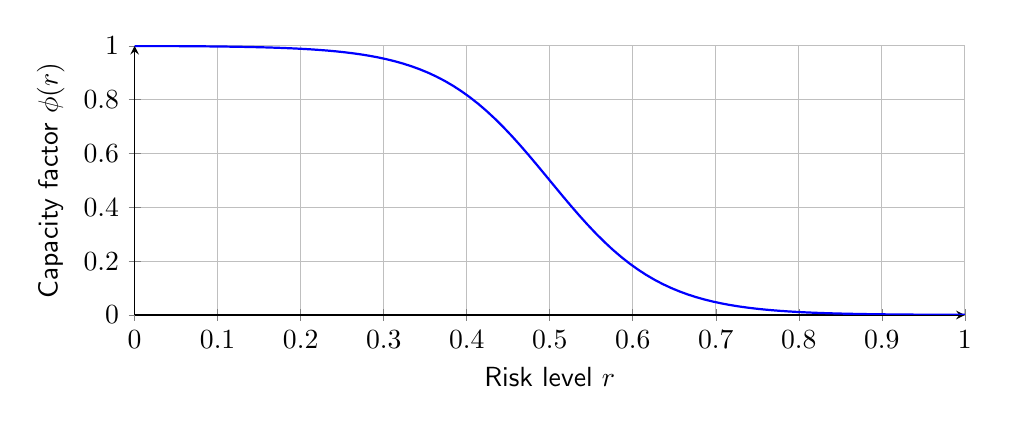
\begin{tikzpicture}
        \begin{axis}[
                width=\columnwidth,
                height=5cm,
                xlabel={Risk level $r$},
                ylabel={Capacity factor $\phi(r)$},
                domain=0:1,
                samples=100,
                grid=major,
                ymin=0, ymax=1,
                xmin=0, xmax=1,
                axis lines=left,
                enlarge x limits=false,
                enlarge y limits=false,
            ]
            \addplot[blue, thick] {1 / (1 + exp(15*(x - 0.5)))};
        \end{axis}
    \end{tikzpicture}
    \caption{\small Sigmoid capacity function $\phi(r)$ modulating effective collateralization based on pool risk level}
    \label{fig:sigmoid-capacity}
\end{figure}

\subsection{Risk Level}
\label{sec:risk-level-calculation}

The risk level $r_M$ quantifies the operational health of pool $M$ by assessing the participation and reliability of its members, with a preference toward established, proven validators. This metric feeds directly into the capacity adjustment function $\phi(r_M)$ defined in equation \ref{eq:risk-sigmoid}, determining the pool's effective collateralization.

DynaFed tracks individual member weights and aggregates them to compute the \textbf{pool-level risk}:

\begin{equation}
    \label{eq:aggr-risk-level}
    r_M = 1 - \frac{\sum_{m \in M} w(m)}{|M|}
\end{equation}

where $w(m)$ is the \textbf{member weight} for member $m$, defined as:

\begin{equation}
    w(m) = \sigma_M \times \psi_M \times \left(\alpha \times s_m + (1-\alpha) \times t_m\right)
\end{equation}

with components:
\begin{itemize}
    \item $\sigma_M \in \{0, 1\}$: state control parameter as defined in section \ref{sec:state-control-parameter}
    \item $\psi_M \in \{0, 1\}$: emergency controller as defined in section \ref{sec:emergency-controller}
    \item $\alpha \in [0.5, 0.7]$: weight parameter balancing recent performance versus long-term tenure
    \item $s_m$: participation score as defined in section \ref{sec:participation-score}
    \item $t_m$: tenure score as defined in section \ref{sec:tenure-score}
\end{itemize}

\subsubsection{State Control Parameter}
\label{sec:state-control-parameter}

The state control parameter $\sigma_M$ acts as an activation gate that prevents premature capacity allocation during the observation window when block samples are insufficient for reliable member scoring. Newly established pools require time to accumulate sufficient data before their participation and tenure scores can meaningfully reflect operational health.

The state control parameter is defined as:

\begin{equation}
    \label{eq:state-control-parameter}
    \sigma_M = \begin{cases}
        0 & \text{if } b - b_0^M < N_{\min} \text{ or } p_M < |M|     \\
        1 & \text{if } b - b_0^M \geq N_{\min} \text{ and } p_M = |M|
    \end{cases}
\end{equation}

where:
\begin{itemize}
    \item $b$: current block height
    \item $b_0^M$: block height when pool $M$ was created (after DKG completion)
    \item $N_{\min}$: minimum observation period (e.g., 100 blocks $\approx$ 10 minutes)
    \item $p_M = |\{m \in M : s_m(b) > 0\}|$: count of members who have submitted at least one FROST proof, where $s_m$ is participation score as described in section \ref{sec:participation-score}.
\end{itemize}

During the observation window ($\sigma_M = 0$), all member weights become zero regardless of their individual participation or tenure scores. This suppresses the influence of high volatility in both $s_m$ and $t_m$ that occurs when few blocks have elapsed. The pool remains in this dormant state until sufficient time has passed to establish reliable scoring patterns.

Once $\sigma_M$ transitions to 1, the pool is considered \textbf{activated} and its risk level directly reflects member performance through the standard risk calculation. Conceptually, a pool is being \textbf{onboarded} when $\sigma_M = 0$ during the observation phase, which forces $r_M = 1$ regardless of individual member scores. A pool is being \textbf{offboarded} or sunset when $\sigma_M = 1$ but $r_M \to 1$ due to member degradation, triggering capacity wind-down through the sigmoid function. This binary state transition ensures a clean separation between the observation phase and normal operational status.

\subsubsection{Emergency Controller}
\label{sec:emergency-controller}

The emergency controller $\psi_M$ provides a critical safety mechanism that forces immediate pool shutdown when the number of active members approaches the FROST signing threshold. While the gradual risk assessment through $\phi(r_M)$ handles normal operational degradation, FROST threshold signatures require a minimum number of functioning members to execute transactions. If a pool degrades to the point where it risks falling below this operational threshold, gradual wind-down is insufficient; the pool must be sunset immediately before it becomes unable to sweep its own funds.

The emergency controller is defined as:

\begin{equation}
    \label{eq:emergency-controller}
    \psi_M = \begin{cases}
        0 & \text{if } A_M < \lceil |M| \times \rho_{\text{safety}} \rceil \\
        1 & \text{otherwise}
    \end{cases}
\end{equation}

where:
\begin{itemize}
    \item $A_M = |\{m \in M : s_m(b) > \theta_{\text{active}}\}|$: count of members exceeding the liveness threshold
    \item $\theta_{\text{active}}$: liveness threshold for considering a member "active" (e.g., 0.8)
    \item $\rho_{\text{safety}} = \frac{t_M}{|M|} + \epsilon_M$: safety ratio relative to FROST threshold
    \item $t_M$: FROST signing threshold for pool $M$ (e.g., 12 for a 12-of-16 multisig)
    \item $\epsilon_M$: collateralization-aware safety buffer
\end{itemize}

The safety buffer $\epsilon_M$ adapts based on pool tier and collateralization status:

\begin{equation}
    \label{eq:safety-buffer}
    \epsilon_M = \begin{cases}
        \epsilon_{\text{strict}} & \text{if Tier 1 or } F_M > C_M     \\
        0                        & \text{if Tier 2 and } F_M \leq C_M
    \end{cases}
\end{equation}

where $\epsilon_{\text{strict}} = 0.125$ provides a safety buffer above the FROST threshold as a fraction of pool size, and $F_M$ and $C_M$ are the pool's current funds and total collateralization as defined in section \ref{sec:collateralization-level}.

\textbf{Design Rationale}: Tier 1 pools and under-collateralized Tier 2 pools maintain strict safety buffers because fund loss is possible if the pool becomes inoperable. Over-collateralized Tier 2 pools use $\epsilon_M = 0$, triggering emergency shutdown only at the actual FROST threshold. This relaxed approach is justified because these pools have full collateral backing on Tier 1. The worst-case failure is service degradation (pegout delays), not fund loss. This provides maximum operational flexibility for hot wallets while the collateral guarantee provides the safety net.

When $\psi_M = 0$, all member weights become zero regardless of individual scores, forcing $r_M = 1$ and consequently $\phi(r_M) \approx 0$. This immediately halts new pegin allocation to the pool and triggers urgent fund sweeping to healthy pools.

\subsubsection{Participation Score}
\label{sec:participation-score}

The participation score $s_m$ measures the recent liveness and responsiveness of member $m$. Members prove their active participation by submitting FROST signature proofs via the NDD as described in section \ref{sec:foundation-layer}. These proofs serve dual purposes: they demonstrate that members possess their key material and are online, actively participating in consensus.

A critical constraint is that FROST proof submission requires the member to be selected as block producer, enabling them to include their proof in the NDD. This means members compete for block production slots not just among pool members $|M|$, but across the entire validator set $N_v$. We assume CometBFT's fair block producer selection guarantees that over sufficient time, every validator has approximately equal opportunity to produce blocks. Members may implement external gossiping mechanisms allowing others to include their proofs on their behalf, which is secure given that FROST proofs are cryptographically signed.

The participation score uses an exponentially weighted moving average (EWMA), similar to the dynamic capacity target in section \ref{sec:dynamic-capacity-target}. This approach is computationally efficient, requires minimal storage, and naturally adapts to changing behavior:

\begin{equation}
    \label{eq:participation-score}
    s_m(b) = \beta \times p_m(b) \times N_v + (1 - \beta) \times s_m(b-1)
\end{equation}

where:
\begin{itemize}
    \item $s_m(b)$: participation score at block height $b$
    \item $p_m(b) \in \{0, 1\}$: proof indicator (1 if member $m$ submitted valid FROST proof in block $b$, 0 otherwise)
    \item $N_v$: total number of validators in the network
    \item $\beta \in [0.001, 0.01]$: smoothing factor controlling responsiveness versus stability
\end{itemize}

The $N_v$ scaling factor normalizes for expected block production frequency, ensuring that members who consistently submit proofs when selected converge to $s_m \approx 1$, while unreliable members decay toward $s_m \approx 0$. The initial condition is $s_m(b_0^M) = 0$, requiring new members to establish their reliability through observed behavior.

The smoothing factor $\beta$ is intentionally small because the EWMA updates every block (every 6 seconds), while individual members produce blocks infrequently at rate $1/N_v$. This ensures the score smooths over multiple block production opportunities rather than reacting to single events.

\subsubsection{Tenure Score}
\label{sec:tenure-score}

The tenure score $t_m$ measures how long a member has been part of an active pool, reflecting establishment and stability within the system. Unlike the participation score which tracks recent performance, tenure captures long-term presence independent of current behavior. This distinction ensures that newly activated members with perfect participation still operate at reduced weight until they prove sustained reliability over time.

Tenure is calculated as the fraction of time elapsed since pool activation, capped at the maturity threshold:

\begin{equation}
    t_m = \min\left(1, \frac{b - b_0^M}{N_{\text{maturity}}}\right)
\end{equation}

where:
\begin{itemize}
    \item $t_m$: tenure score for member $m$
    \item $b$: current block height
    \item $b_0^M$: block height when pool $M$ was activated
    \item $N_{\text{maturity}}$: maturity threshold (e.g., 14,400 blocks $\approx$ 24 hours)
\end{itemize}

All members of pool $M$ share the same tenure score since it depends only on pool activation time, not individual member behavior. A newly activated pool begins with $t_m = 0$ for all members, reaching full tenure credit ($t_m = 1$) after $N_{\text{maturity}}$ blocks of operation. This creates the "gradually, then suddenly" capacity ramp described in section \ref{sec:risk-assessment}, where new pools start with limited effective collateralization that grows as they demonstrate sustained operational stability.

The tenure score is computationally trivial, requiring only two block height values and basic arithmetic, and provides the timespan that complements the performance-based participation score in the composite member weight.

\section{The Foundation Layer}
\label{sec:foundation-layer}

The Foundation Layer is the central coordination component that orchestrates Botanix's multisig federation system. It integrates several subsystems described throughout this paper:

\begin{itemize}
    \item \textbf{Pool Management} (section \ref{sec:pool-management}): Pegin and pegout allocation across the two-tier federation architecture
    \item \textbf{Risk Assessment} (section \ref{sec:risk-assessment}): Pool health monitoring and lifecycle management
    \item \textbf{Bitcoin Fork Awareness} (section \ref{sec:bitcoin-fork-awareness}): Tracking pegout proposals across Bitcoin's probabilistic finality model
    \item \textbf{State Commitments} (section \ref{sec:foundation-state-proof}): Cryptographic proofs enabling deterministic validation across all validators
\end{itemize}

As described in section \ref{sec:overview}, the Foundation Layer produces the \textbf{Non-Deterministic Data (NDD)} $\gamma$ included in every block. While the NDD is constructed subjectively by the block producer, all validators verify its contents against the Foundation Layer's consensus rules. This design enables off-chain coordination, such as FROST signing rounds and pegout batching, to be anchored on-chain without requiring validators to track external state.

The NDD supports the following message types:

\begin{itemize}
    \item \textbf{Pegout Proposal} (section~\ref{sec:pegout-proposals}): Submits a new proposal, upgrades an existing proposal (section~\ref{sec:pegout-proposal-upgrade}), or cancels a proposal (section~\ref{sec:pegout-proposal-cancellation}). This message type also covers fund sweeping during pool migration and sunsetting operations.
    \item \textbf{Bitcoin Header} (section~\ref{sec:bitcoin-fork-awareness}): Registers a new Bitcoin block header, validated by verifying that its hash falls below the Proof-of-Work target and that its parent is already known to the Foundation Layer.
    \item \textbf{Bitcoin Transaction} (section~\ref{sec:bitcoin-fork-awareness}): Associates a pegout proposal with a registered Bitcoin block via a Merkle inclusion proof, enabling finality tracking.
    \item \textbf{FROST Signature Proof} (section~\ref{sec:participation-score}): Demonstrates that a pool member possesses valid key material and is actively participating in consensus. These proofs feed into the participation score used for risk assessment.
\end{itemize}

\textbf{Note}: The NDD message format is designed for extensibility. Future protocol versions may introduce additional message types for staking, slashing, and other consensus-critical operations.

The Foundation Layer operates on a critical principle: it treats all input as potentially malicious, verifies input through cryptographic proofs, and makes decisions based solely on provided inputs without requiring access to external networks. This self-contained verification model ensures that validators reach consensus on Foundation state without relying on external oracles or subjective observations of the Bitcoin network.

\subsection{Pegout Proposals}
\label{sec:pegout-proposals}

Bitcoin uses a probabilistic finality system rather than deterministic finality. We assume that after sufficient time and spent resources, a reorganization becomes economically unviable if not practically impossible. However, given this probabilistic nature and competing blocks, the Foundation Layer must be fork-aware and consider various scenarios:

\begin{itemize}
    \item A Bitcoin transaction can be rejected by nodes or miners even though it's valid under consensus rules. For example, if fee rates are unattractive, local mempool policies differ, or other configurable parameters aren't met. Different nodes and miners may have conflicting views on which transactions to propagate or include.
    \item A previously rejected transaction might later be picked up and propagated, potentially remaining unconfirmed for extended periods.
    \item A Bitcoin transaction might need to be accelerated or replaced by DynaFed. There's no guarantee that a replacement transaction will take precedence over the original.
    \item Even if a transaction is widely propagated, miners may choose not to include it in a block for arbitrary reasons. Fundamentally, there's no way to deterministically or objectively determine whether a Bitcoin transaction will be mined.
\end{itemize}

In our Foundation Layer model, \textbf{UTXO reuse} becomes the key safeguard that anchors our entire system, especially when integrated with the TEE/TEM architecture. This dramatically reduces state management complexity. Pegouts are categorized in one of two states:

\begin{itemize}
    \item \textbf{Unassigned}: Fresh pegouts that have been triggered on the Botanix EVM but not yet included in any proposal.
    \item \textbf{Proposed}: Pegouts that are part of a proposed Bitcoin transaction, coupled with the selected UTXO(s).
\end{itemize}

Critically, a pegout proposal must be submitted to the Foundation Layer before multisig members sign the PSBT. The coordinator or representative of a multisig federation must first include their proposal in the Foundation Layer, and only then will other members accept signing the proposal off-chain. That proposal remains in the Proposed state until it's finalized, or gets removed by a competing transaction being finalized first.

The Foundation Layer enforces a crucial invariant: \textbf{pegouts and UTXOs in a proposal are tightly coupled}. The layer will only allow replacing or updating proposals if the updated (competing) proposal reuses at least one UTXO from the original. This means that if multiple Bitcoin transactions all share at least one UTXO, we have a core guarantee that \textbf{only one will become probabilistically finalized}, the others will fail due to the spent UTXO. This elegant property handles forks, replacements, and race conditions without complex state tracking.

\subsubsection{Updating Proposal}
\label{sec:pegout-proposal-upgrade}

Federation representatives may need to update an existing pegout proposal to adjust transaction parameters such as fee rates, consolidate additional pegouts, or respond to changing mempool conditions. The Foundation Layer supports proposal updates through a replacement mechanism anchored by UTXO reuse.

To update a proposal, the representative submits a new proposal that satisfies two requirements:

\begin{itemize}
    \item \textbf{UTXO continuity}: The new proposal must reuse at least one UTXO from the original proposal, establishing a link between the two versions
    \item \textbf{Federation authorization}: Only the original proposing federation can submit updates, verified through the federation identifier
\end{itemize}

This mechanism enables common operations such as:

\begin{itemize}
    \item \textbf{Fee adjustment}: Replacing a low-fee transaction with a higher-fee version (Replace-By-Fee)
    \item \textbf{Pegout consolidation}: Including additional pending pegouts in an updated transaction
    \item \textbf{UTXO optimization}: Adjusting input selection for better transaction efficiency
\end{itemize}

The UTXO reuse property ensures that only one version of the proposal can eventually finalize on the Bitcoin blockchain. When the updated transaction confirms, the original proposal is automatically invalidated through the spent UTXO, preventing any possibility of double-execution. The Foundation Layer tracks both proposals until one achieves finality, at which point the competing version is removed from state.

\subsubsection{Cancelling Proposal}
\label{sec:pegout-proposal-cancellation}

Circumstances may require canceling a pegout proposal without fulfilling its original pegouts. The Foundation Layer supports cancellation through the same UTXO reuse mechanism used for updates, with two primary approaches:

\begin{itemize}
    \item \textbf{Consolidation}: The federation submits a transaction that spends the proposal's UTXOs back to an address it controls, without including any pegout outputs. This effectively "consumes" the UTXOs while returning funds to the federation.

    \item \textbf{Replacement}: The federation submits an entirely different proposal that reuses at least one UTXO from the original. When the replacement achieves finality, the original proposal is invalidated through the spent UTXO.
\end{itemize}

When the cancellation transaction achieves finality, the Foundation Layer automatically returns the original pegouts to the unassigned state, making them available for inclusion in future proposals. This recovery mechanism ensures that user withdrawal requests are never permanently lost due to proposal failures. They simply re-enter the queue for the next available federation to fulfill.

\subsection{Foundation State Proof}
\label{sec:foundation-state-proof}

The Foundation Layer maintains a cryptographic proof of its complete state, enabling deterministic validation across all consensus participants. This state proof commits to four key components: context metadata, the commitment trie root, tracked Bitcoin headers, and auxiliary events that enable efficient state indexing and reconstruction.

The commitment trie root $r_{\text{trie}}$ (section \ref{sec:foundation-state-proof-structure}) employs the Base-16 Modified Patricia Merkle Tree as implemented by Parity Technologies\footnote{\url{https://github.com/paritytech/trie}} to construct and validate state proofs. The architecture separates data storage from commitment construction: the trie operates exclusively on cryptographic hashes of key-value pairs, maintaining independence from the underlying database implementation.

The system supports any key-value database backend (e.g., RocksDB, MDBX) that provides atomic commit and rollback mechanisms. These transactional guarantees must be supplied by the database layer and fall outside the scope of the trie commitment specification itself.

\subsubsection{State Proof Structure}
\label{sec:foundation-state-proof-structure}

The complete Foundation state proof is represented as:

\begin{equation}
    \mathcal{F}^{\Phi} = (\text{context}, r_{\text{trie}}, \text{headers}, \text{events})
\end{equation}

where:
\begin{itemize}
    \item $\text{context}$: Protocol context and version metadata (section \ref{sec:foundation-context-metadata})
    \item $r_{\text{trie}}$: 32-byte commitment trie root as produced by the Tree implementation
    \item $\text{headers}$: Set of tracked Bitcoin block hashes
    \item $\text{events}$: Sequence of auxiliary events (section \ref{sec:foundation-aux-events}) for state reconstruction
\end{itemize}

\subsubsection{Context Metadata}
\label{sec:foundation-context-metadata}

The context provides version information and is primarily reserved for future protocol extensions:

\begin{equation}
    \text{context} = (\text{height})
\end{equation}

where $\text{height}$ is the current Botanix block height.

\subsubsection{Auxiliary Events}
\label{sec:foundation-aux-events}

Auxiliary events provide an efficient event log enabling state reconstruction and indexing without reprocessing the entire commitment validation sequence.

The following event types are recorded:

\begin{itemize}
    \item \textbf{Initiated Pegout}: Records a newly initiated pegout available for spending, including the pegout identifier and the list of candidate federations qualified to fulfill it.
    \item \textbf{Submitted Proposal}: Records a newly submitted pegout proposal, capturing the complete proposal entry.
    \item \textbf{New Bitcoin Header}: Records a Bitcoin block header being tracked by the Foundation Layer.
    \item \textbf{Registered Bitcoin Transaction}: Records a Bitcoin transaction registration, associating a transaction with its containing block and the set of pegouts it fulfills.
    \item \textbf{Finalized Bitcoin Header}: Records a finalized Bitcoin block along with the set of pegout identifiers that have reached finality.
    \item \textbf{Orphaned Bitcoin Header}: Records an orphaned Bitcoin block along with the set of pegout identifiers that have been returned to unassigned (spendable) state.
\end{itemize}


\clearpage
\section{Appendix}

This appendix provides technical details and derivations referenced throughout the main text.

\subsection{DKG: Message Complexity}
\label{appendix:dkg-message-complexity}

This appendix provides a detailed breakdown of the message complexity for FROST DKG setup, as referenced in section \ref{sec:frost-challenge}. We measure the number of \textbf{messages that must be sent over the wire}, where the coordinator functions not only as a participant in the multisig setup, but also as a message forwarder/router.

We examine two approaches: \textbf{with and without message bundling}. The key difference is that with bundling, the coordinator waits until all messages per round are received, then sends all necessary packages to each non-coordinator as a single bundle. This applies to both received and sent messages in round 2. Without bundling, the coordinator forwards each package individually as they are received.

\subsubsection{Comparison}

Bundling reduces message complexity from quadratic $O(n^2)$ to linear $O(n)$:

\begin{itemize}
    \item \textbf{Without bundling}: $3n^2-5n+2$ messages
    \item \textbf{With bundling}: $4n-4$ messages
\end{itemize}

For example, with $n=32$ participants:
\begin{itemize}
    \item Without bundling: 2,914 messages
    \item With bundling: 124 messages
\end{itemize}

With $n=64$ participants:
\begin{itemize}
    \item Without bundling: 11,970 messages
    \item With bundling: 252 messages
\end{itemize}

And with $n=128$ participants:
\begin{itemize}
    \item Without bundling: 48,514 messages
    \item With bundling: 508 messages
\end{itemize}

Bundling represents a \textbf{significant reduction} in message count, though at the cost of larger individual message sizes.

\subsubsection{With Bundling}

The coordinator waits until all messages per round are received, then sends all necessary packages to each non-coordinator as a \textbf{single bundle}. This applies to both round 1 and round 2.

\paragraph{Each Round}

Each non-coordinator sends their package to the coordinator. Since the coordinator already has their own package, they receive the following number of messages over the wire:

\[n-1\]

The coordinator then forwards all packages as a single bundle to each of the $n-1$ non-coordinator member (excluding themselves), sending:

\[n-1\]

Total messages per round:

\[(n-1)+(n-1) = 2n-2\]

\paragraph{Total}

The total message complexity across both round 1 and round 2:

\begin{equation}
\begin{aligned}
2\times (2n-2)\\ = 4n-4
\end{aligned}
\end{equation}

\subsubsection{Without Bundling}

The coordinator forwards each package individually rather than bundling them together. While this keeps individual message sizes smaller, it significantly increases the total message count.

\paragraph{Round 1}

Each non-coordinator sends their package to the coordinator. Since the coordinator already has their own package, they receive the following number of messages over the wire:

\[n-1\]

The coordinator forwards each of the $n-1$ packages to each of the $n-1$ non-coordinators (excluding themselves), sending:

\[(n-1)(n-1) = n^2-2n+1\]

Total messages for round 1:

\[(n-1)+(n^2-2n+1) = n^2-n\]

\paragraph{Round 2}

Each non-coordinator creates individual packages for each other member (excluding themselves), sending $n-1$ packages to the coordinator. Since the coordinator already has their own packages, they receive the following number of messages over the wire:

\[(n-1)(n-1) = n^2-2n+1\]

The coordinator then forwards each individual package to its corresponding recipient (excluding themselves), sending:

\[(n-1)(n-1) = n^2-2n+1\]

Total messages for round 2:

\[(n^2-2n+1)+(n^2-2n+1) = 2n^2-4n+2\]

\paragraph{Total}

The total message complexity across both round 1 and round 2:

\begin{equation}
\begin{aligned}
(n^2-n)+(2n^2-4n+2)\\= 3n^2-5n+2
\end{aligned}
\end{equation}

\subsection{Block Tree}
\label{sec:block-tree}

The block tree maintains a lightweight representation of the Bitcoin blockchain, tracking competing forks and automatically pruning blocks as they reach sufficient confirmation depth. This structure enables deterministic fork resolution across all Botanix validators without requiring full Bitcoin node synchronization.

The block tree serves two critical functions:
\begin{itemize}
    \item \textbf{Fork Detection}: Identifies competing Bitcoin chains and preserves unresolved forks until one becomes canonical
    \item \textbf{Automatic Pruning}: Removes blocks that have either reached finality or been orphaned, preventing unbounded memory growth
\end{itemize}

The theoretical motivation for Bitcoin fork awareness and its role in pegout finality is described in section \ref{sec:bitcoin-fork-awareness}. This section provides the technical specification for the block tree data structure and its operations.

\subsubsection{Core Definitions}

Let $B$ denote the set of all blocks in the tree, where each block $b \in B$ has:
\begin{itemize}
    \item A block hash $h(b)$
    \item A parent hash $p(b)$
    \item A set of children $C(b) \subseteq B$
    \item A relative height $r(b) \in \mathbb{N}$, defined as the distance from the tree's root (elder)
\end{itemize}

We define:
\begin{itemize}
    \item $T \subseteq B$: the set of tips (blocks with no children, i.e., $C(b) = \emptyset$)
    \item $e \in B$: the elder (oldest retained block with $r(e) = \min_{b \in B} r(b)$)
    \item $h_{best} = \max_{b \in B} r(b)$: the best (maximum) height in the tree
    \item $d_{conf}$: the confirmation depth parameter (minimum 3)
\end{itemize}

\subsubsection{Block Insertion and Pruning}
\label{btc:insert-prune}

The block insertion operation processes a new Bitcoin block and automatically prunes finalized and orphaned blocks:

\begin{equation}
\Pi(b_{new}) \rightarrow \{\text{fate}(b_1), \text{fate}(b_2), \ldots\}
\end{equation}

This operation inserts the new block, performs two-phase pruning, and returns the possibly empty set of pruned blocks with their classifications as defined in section \ref{sec:fork-block-classification}.

When inserting a new block $b_{new}$ with parent $b_{parent}$:

\begin{enumerate}
    \item \text{Height assignment}:
    
    \[r(b_{new}) = r(b_{parent}) + 1\]
    
    \item \text{Relationship update}:
    
    \[C(b_{parent}) := C(b_{parent}) \cup \{b_{new}\}\]
    
    \item \text{Tip update}:

    \[T := (T \setminus \{b_{parent}\}) \cup \{b_{new}\}\]
    
    \item \text{Best height update}:
    
    \[\textit{If } r(b_{new}) > h_{best}\textit{, then } h_{best} := r(b_{new})\]
\end{enumerate}

Following insertion, the tree is automatically pruned in two phases:

\begin{enumerate}
    \item \textbf{Backward pruning}: Remove orphaned forks from tips as defined in section \ref{sec:fork-backward-pruning}, enabling forward progress
    \item \textbf{Forward pruning}: Remove finalized blocks from the elder as defined in section \ref{sec:fork-forward-pruning}, advancing the elder forward
\end{enumerate}

This two-phase approach ensures that orphaned forks don't block forward pruning of the canonical chain, that unresolved forks prevent premature finalization, and that the elder always represents the oldest block in any active chain.

\subsubsection{Pruning Criteria}

A block $b$ becomes eligible for pruning when:

\begin{equation}
r(b) \leq h_{best} - (d_{conf} - 1)
\end{equation}

This defines the \textbf{pruning threshold}:
\begin{equation}
h_{prune} = h_{best} - (d_{conf} - 1)
\end{equation}

\subsubsection{Backward Pruning (Orphaned)}
\label{sec:fork-backward-pruning}

For each tip $t \in T$, the algorithm checks if the tip represents an orphaned fork by traversing backward toward the elder. A tip $t$ is orphaned if:

\begin{equation}
r(t) \leq h_{prune}
\end{equation}

The backward traversal removes parent-child relationships and prunes childless blocks:

\begin{enumerate}
    \item For a block $b$ with child $c$ (or tip if $c = \emptyset$):
    \begin{itemize}
        \item \textit{If} $r(b) \leq h_{prune}$ and a child exists:
        
        \[C(b) := C(b) \setminus \{c\}\]
        
        \item \textit{If} $C(b) = \emptyset$ after removal: remove $b$ from $B$ and classify as \textbf{orphaned}
        \item Recursively process parent $p(b)$
    \end{itemize}
    
    \item Termination occurs when:
    \begin{itemize}
        \item $r(b) > h_{prune}$ (block is too recent), or
        \item The parent has been reached that still has other children: $C(b) \neq \emptyset$
    \end{itemize}
\end{enumerate}

\subsubsection{Forward Pruning (Finalized)}
\label{sec:fork-forward-pruning}

Starting from the elder $e$, the algorithm prunes finalized blocks that satisfy all of the following conditions:

\begin{enumerate}
    \item \text{Depth condition}:
    
    \[r(e) \leq h_{prune}\]
    
    \item \text{No fork condition (exactly one child)}:
    
    \[|C(e)| = 1\]
\end{enumerate}

The forward pruning process recursively follows the chain:

\begin{equation}
e' = \begin{cases}
c & \text{if } r(e) \leq h_{prune} \land |C(e)| = 1 \\
e & \text{otherwise}
\end{cases}
\end{equation}

where $c$ is the unique child in $C(e)$. Each pruned block is classified as \textbf{finalized}.

The algorithm terminates when it encounters a block that either:

\begin{itemize}
    \item Is above the pruning threshold: $r(e) > h_{prune}$, or
    \item Has multiple children: $|C(e)| > 1$, indicating an unresolved fork
\end{itemize}

\subsubsection{Block Classification}
\label{sec:fork-block-classification}

Pruned blocks are classified as:

\begin{equation}
\text{fate}(b) = \begin{cases}
\text{Finalized} & \text{if pruned via forward traversal} \\
\text{Orphaned} & \text{if pruned via backward traversal}
\end{cases}
\end{equation}

This classification determines the handling of associated pegouts: finalized blocks indicate permanent confirmation, while orphaned blocks require returning pegouts to the pending set.

\end{document}